\subsubsection*{La velocità istantanea}

Fino ad ora, abbiamo quasi utilizzato sempre il concetto di {\slshape velocità` media}, intesa come proprietà associata a una {\slshape coppia} di eventi.\newline
Tuttavia, a volte serve pensare alla velocità come proprietà dello stato di moto di un singolo evento e si parla, in questo caso, di {\bf velocità istantanea}.\newline

Il concetto di velocità istantanea diventa realmente utile quando si studia un moto vario, dove la velocità cambia istante per istante. Quando cioè è possibile ritenere che due istanti diversi, per quanto ravvicinati nel tempo, possano avere
delle velocità diverse.\newline

L’uso del concetto di velocità istantanea, però, non è del tutto immediato e richiede un po’ di riflessione.
La velocità si misura dividendo uno spostamento per un intervallo temporale. Un singolo istante, invece, è un punto nel tempo, che non corrisponde ad alcun intervallo e a cui si può` associare una sola posizione.\newline

Pensiamo a un ciclista che transita sul traguardo alla velocità di 50 chilometri orari. Avrebbe senso domandare: {\slshape Quanto spazio percorre il ciclista nel preciso istante in cui tocca il traguardo?} Chiaramente no. Il transito, infatti, avviene
ad una determinata velocità ma, immediatamente dopo, l’atleta rilascia i pedali e comicia a rallentare. Se volessimo capire quanto spazio dopo il traguardo sia stato percorso in venti secondi, non saremmo in grado di esprimere nessuna previsione. Se però ci limitiamo a ragionare per intervalli di tempo più brevi, ci accorgiamo di poter avanzare delle stime meno grossolane. Proviamo a chiederci, ad esempio, quanto spazio viene percorso dal ciclista nel primo secondo.
Trattandosi di un tempo molto breve, potremmo supporrre che la bicicletta abbia rallentato pochissimo, e potremmo avanzare l’ipotesi di osservare, sia pure per un solo secondo, un moto a velocità costante. Cinquanta chilometri all’ora corrisponde a circa undici metri al secondo. Dunque potremmo immaginare che il ciclista si trovi, dopo un secondo, a circa undici metri dietro al traguardo.\newline

Se ripetiamo lo stesso ragionamento per tempi ancora più brevi, otterremmo risultati ancora più convincenti, cioè affetti da un errore più piccolo. In generale, dire che un oggetto possiede una certa velocità istantanea, significa affermare che considerando un intervallo di tempo abbastanza piccolo, si può valutare lo spazio percorso dalla moltiplicazione della velocità data per l’intervallo di tempo, con errore trascurabile, come se stessimo ossservando un moto a velocità costante.

Proviamo ora ad applicare questa idea a un problema più complesso. Immaginiamo che il ciclista precedente si fermi, dopo l’arrivo, in trenta secondi, frenando in modo uniforme.

Per rappresentare graficamente il movimento, possiamo considerare la figura seguente:

\begin{figure}[H]
 \centering
 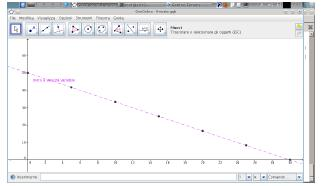
\includegraphics[width=.7\textwidth]{../immagini/frenataUniforme.jpeg}
 % podista.png
 %\label{fig:il grafico velocità tempo di un moto costante}
\end{figure}

Questa curva ci mostra che stiamo osservando un movimento a velocità sempre più lento. Ovvero, un movimento nel quale, a parità di intervallo di tempo, vengono coperti spazi sempre più brevi. Per rappresentare graficamente questa idea, conviene tracciare, intorno alla retta obliqua che rappresenta il moto, una linea spezzata, {\slshape costante a tratti}, come quella nella figura successiva:

\begin{figure}[H]
 \centering
 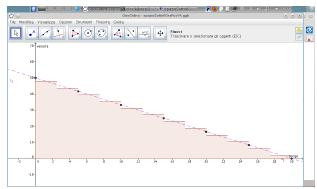
\includegraphics[width=.7\textwidth]{../immagini/scaletta.jpeg}
 % podista.png
 %\label{fig:il grafico velocità tempo di un moto costante}
\end{figure}

In questa immagine, la curva spezzata è un’{\slshape approssimazione} del moto reale. Un’approssimazione è un modello diverso da quello reale, ma costruito con una tecnica tale da avvicinarsi alla realtà con la precisione desiderata. Nell’esempio, il moto è stato suddiviso in dodici intervalli, ma se la suddivisione fosse stata più raffinata, si sarebbe ottenuta una spezzata ancora più simile alla curva originale.\newline
Se osserviamo i singoli rettangoli colorati, sotto ad ogni tratto orizzontale, possiamo osservare che l’area di ciascuno di essi possiede il significato cinematico di spazio percorso. Sapendo che la nostra osservazione è cominciata esattamente nell’istante in cui il ciclista transitava sotto il traguardo, possiamo ricavare dalla curva v-t la posizione esatta del ciclista in ogni istante del proprio moto.\newline

Possiamo cioè dedurre la curva spazio-tempo del moto, che assume l’aspetto di una parabola, come nell’immagine sotto:

\begin{figure}[H]
 \centering
 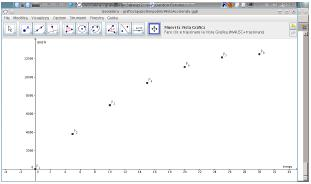
\includegraphics[width=.7\textwidth]{../immagini/curvaSpazioTempo.jpeg}
 % podista.png
 %\label{fig:il grafico velocità tempo di un moto costante}
\end{figure}


L'ordinata di ciscun evento in questa immagine è determinato sommando le aree in rosa della curva velocità tempo. Per esprimere i dati in metri, inoltre, è stato necessario convertire le velocità da chilometri all’ora a metri al secondo.
Nell’immagine si osserva immediatamente che i punti non sono più disposti lungo una linea retta, ma che gli incrementi tra due valori equispaziati nel tempo diminuiscono progressivamente. Questo accade proprio perché la curva velocità tempo osservata dalla quale è stato derivato il grafico è decrescente.\newline

Naturalmente, questa osservazione può essere utilizzata per ragionare nella direzione inversa.\newline
Immaginiamo di produrre una curva sperimentale spazio-tempo di un moto e di voler ricavare da essa un grafico velocità tempo. In questo caso, saremmo interessati a rilevare, per ogni coppia di eventi, il valore della velocità media che, graficamente, è rappresentato dall’inclinazione della retta li congiunge. Questa velocità media sarà un valore diverso per ogni scelta della coppia di punti.
Tuttavia, se osserviamo un insieme di coppie sufficientemente ravvicinate nel tempo, ci viene spontaneo assumere che i valori calcolati delle velocità medie manifestino piccoli cambiamenti, intorno a un determinato valore di riferimento.
Pensandoci ancora meglio, ci possiamo accorgere che questo valore si avvicina al coefficiente angolare della retta tangente alla curva negli estremi dell’intervallo considerato. Questo accade se l’intervallo di tempo tra gli eventi è sufficentemente piccolo da poter essere considerato come un unico istante. Il valore corrispondente della velocità, in questo caso, assume il nome di {\bf velocità istantanea}\footnote {a rigore, questa operazione andrebbe descritta da un processo di limite, ma qui usiamo una descrizione semplificata di tipo qualitativo. seguirà immagine ...}.

